\documentclass[1p]{elsarticle_modified}
%\bibliographystyle{elsarticle-num}

%\usepackage[colorlinks]{hyperref}
%\usepackage{abbrmath_seonhwa} %\Abb, \Ascr, \Acal ,\Abf, \Afrak
\usepackage{amsfonts}
\usepackage{amssymb}
\usepackage{amsmath}
\usepackage{amsthm}
\usepackage{scalefnt}
\usepackage{amsbsy}
\usepackage{kotex}
\usepackage{caption}
\usepackage{subfig}
\usepackage{color}
\usepackage{graphicx}
\usepackage{xcolor} %% white, black, red, green, blue, cyan, magenta, yellow
\usepackage{float}
\usepackage{setspace}
\usepackage{hyperref}

\usepackage{tikz}
\usetikzlibrary{arrows}

\usepackage{multirow}
\usepackage{array} % fixed length table
\usepackage{hhline}

%%%%%%%%%%%%%%%%%%%%%
\makeatletter
\renewcommand*\env@matrix[1][\arraystretch]{%
	\edef\arraystretch{#1}%
	\hskip -\arraycolsep
	\let\@ifnextchar\new@ifnextchar
	\array{*\c@MaxMatrixCols c}}
\makeatother %https://tex.stackexchange.com/questions/14071/how-can-i-increase-the-line-spacing-in-a-matrix
%%%%%%%%%%%%%%%

\usepackage[normalem]{ulem}

\newcommand{\msout}[1]{\ifmmode\text{\sout{\ensuremath{#1}}}\else\sout{#1}\fi}
%SOURCE: \msout is \stkout macro in https://tex.stackexchange.com/questions/20609/strikeout-in-math-mode

\newcommand{\cancel}[1]{
	\ifmmode
	{\color{red}\msout{#1}}
	\else
	{\color{red}\sout{#1}}
	\fi
}

\newcommand{\add}[1]{
	{\color{blue}\uwave{#1}}
}

\newcommand{\replace}[2]{
	\ifmmode
	{\color{red}\msout{#1}}{\color{blue}\uwave{#2}}
	\else
	{\color{red}\sout{#1}}{\color{blue}\uwave{#2}}
	\fi
}

\newcommand{\Sol}{\mathcal{S}} %segment
\newcommand{\D}{D} %diagram
\newcommand{\A}{\mathcal{A}} %arc


%%%%%%%%%%%%%%%%%%%%%%%%%%%%%5 test

\def\sl{\operatorname{\textup{SL}}(2,\Cbb)}
\def\psl{\operatorname{\textup{PSL}}(2,\Cbb)}
\def\quan{\mkern 1mu \triangleright \mkern 1mu}

\theoremstyle{definition}
\newtheorem{thm}{Theorem}[section]
\newtheorem{prop}[thm]{Proposition}
\newtheorem{lem}[thm]{Lemma}
\newtheorem{ques}[thm]{Question}
\newtheorem{cor}[thm]{Corollary}
\newtheorem{defn}[thm]{Definition}
\newtheorem{exam}[thm]{Example}
\newtheorem{rmk}[thm]{Remark}
\newtheorem{alg}[thm]{Algorithm}

\newcommand{\I}{\sqrt{-1}}
\begin{document}

%\begin{frontmatter}
%
%\title{Boundary parabolic representations of knots up to 8 crossings}
%
%%% Group authors per affiliation:
%\author{Yunhi Cho} 
%\address{Department of Mathematics, University of Seoul, Seoul, Korea}
%\ead{yhcho@uos.ac.kr}
%
%
%\author{Seonhwa Kim} %\fnref{s_kim}}
%\address{Center for Geometry and Physics, Institute for Basic Science, Pohang, 37673, Korea}
%\ead{ryeona17@ibs.re.kr}
%
%\author{Hyuk Kim}
%\address{Department of Mathematical Sciences, Seoul National University, Seoul 08826, Korea}
%\ead{hyukkim@snu.ac.kr}
%
%\author{Seokbeom Yoon}
%\address{Department of Mathematical Sciences, Seoul National University, Seoul, 08826,  Korea}
%\ead{sbyoon15@snu.ac.kr}
%
%\begin{abstract}
%We find all boundary parabolic representation of knots up to 8 crossings.
%
%\end{abstract}
%\begin{keyword}
%    \MSC[2010] 57M25 
%\end{keyword}
%
%\end{frontmatter}

%\linenumbers
%\tableofcontents
%
\newcommand\colored[1]{\textcolor{white}{\rule[-0.35ex]{0.8em}{1.4ex}}\kern-0.8em\color{red} #1}%
%\newcommand\colored[1]{\textcolor{white}{ #1}\kern-2.17ex	\textcolor{white}{ #1}\kern-1.81ex	\textcolor{white}{ #1}\kern-2.15ex\color{red}#1	}

{\Large $\underline{12a_{0353}~(K12a_{0353})}$}

\setlength{\tabcolsep}{10pt}
\renewcommand{\arraystretch}{1.6}
\vspace{1cm}\begin{tabular}{m{100pt}>{\centering\arraybackslash}m{274pt}}
\multirow{5}{120pt}{
	\centering
	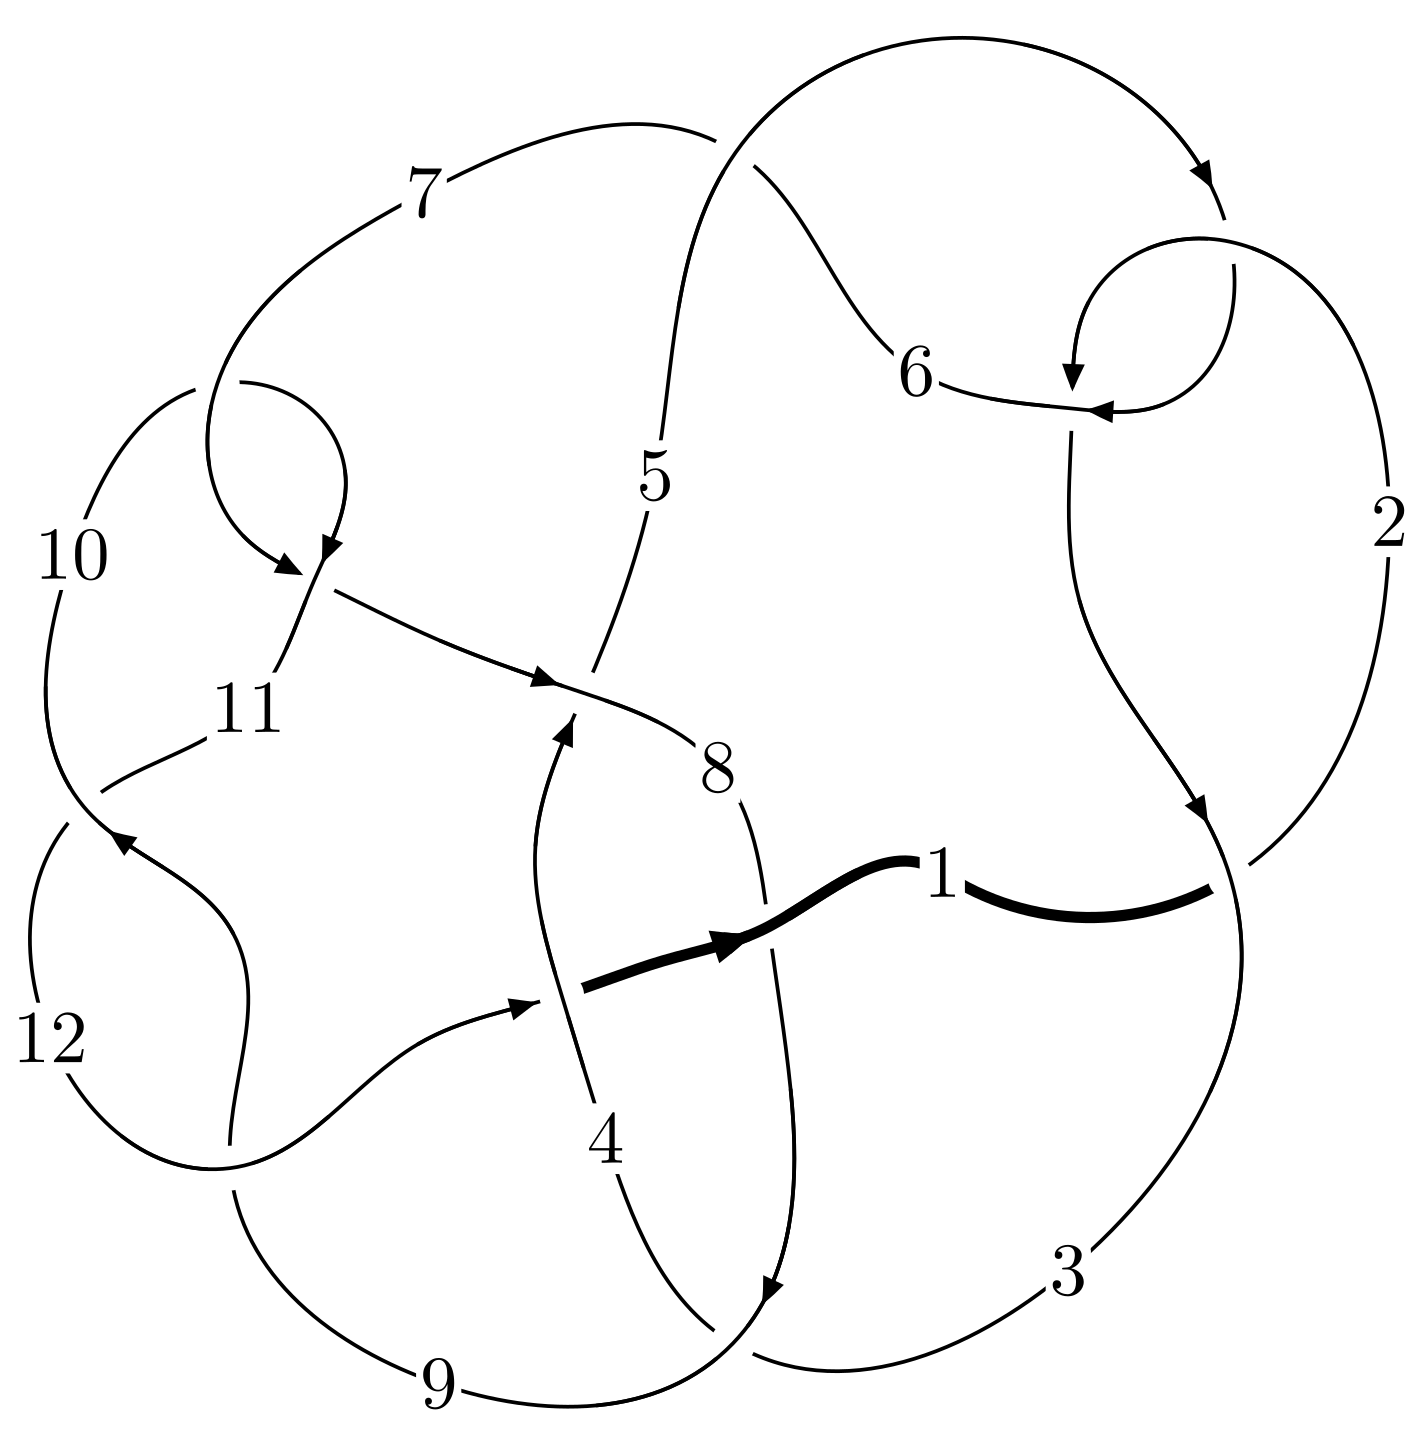
\includegraphics[width=112pt]{../../../GIT/diagram.site/Diagrams/png/1154_12a_0353.png}\\
\ \ \ A knot diagram\footnotemark}&
\allowdisplaybreaks
\textbf{Linearized knot diagam} \\
\cline{2-2}
 &
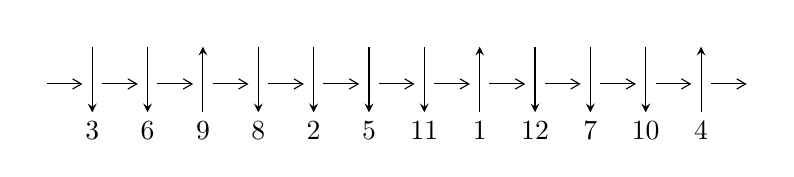
\begin{tikzpicture}[x=20pt, y=17pt]
	% nodes
	\node (C0) at (0, 0) {};
	\node (C1) at (1, 0) {};
	\node (C1U) at (1, +1) {};
	\node (C1D) at (1, -1) {3};

	\node (C2) at (2, 0) {};
	\node (C2U) at (2, +1) {};
	\node (C2D) at (2, -1) {6};

	\node (C3) at (3, 0) {};
	\node (C3U) at (3, +1) {};
	\node (C3D) at (3, -1) {9};

	\node (C4) at (4, 0) {};
	\node (C4U) at (4, +1) {};
	\node (C4D) at (4, -1) {8};

	\node (C5) at (5, 0) {};
	\node (C5U) at (5, +1) {};
	\node (C5D) at (5, -1) {2};

	\node (C6) at (6, 0) {};
	\node (C6U) at (6, +1) {};
	\node (C6D) at (6, -1) {5};

	\node (C7) at (7, 0) {};
	\node (C7U) at (7, +1) {};
	\node (C7D) at (7, -1) {11};

	\node (C8) at (8, 0) {};
	\node (C8U) at (8, +1) {};
	\node (C8D) at (8, -1) {1};

	\node (C9) at (9, 0) {};
	\node (C9U) at (9, +1) {};
	\node (C9D) at (9, -1) {12};

	\node (C10) at (10, 0) {};
	\node (C10U) at (10, +1) {};
	\node (C10D) at (10, -1) {7};

	\node (C11) at (11, 0) {};
	\node (C11U) at (11, +1) {};
	\node (C11D) at (11, -1) {10};

	\node (C12) at (12, 0) {};
	\node (C12U) at (12, +1) {};
	\node (C12D) at (12, -1) {4};
	\node (C13) at (13, 0) {};

	% arrows
	\draw[->,>={angle 60}]
	(C0) edge (C1) (C1) edge (C2) (C2) edge (C3) (C3) edge (C4) (C4) edge (C5) (C5) edge (C6) (C6) edge (C7) (C7) edge (C8) (C8) edge (C9) (C9) edge (C10) (C10) edge (C11) (C11) edge (C12) (C12) edge (C13) ;	\draw[->,>=stealth]
	(C1U) edge (C1D) (C2U) edge (C2D) (C3D) edge (C3U) (C4U) edge (C4D) (C5U) edge (C5D) (C6U) edge (C6D) (C7U) edge (C7D) (C8D) edge (C8U) (C9U) edge (C9D) (C10U) edge (C10D) (C11U) edge (C11D) (C12D) edge (C12U) ;
	\end{tikzpicture} \\
\hhline{~~} \\& 
\textbf{Solving Sequence} \\ \cline{2-2} 
 &
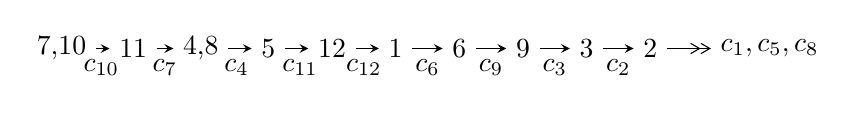
\begin{tikzpicture}[x=23pt, y=7pt]
	% node
	\node (A0) at (-1/8, 0) {7,10};
	\node (A1) at (1, 0) {11};
	\node (A2) at (33/16, 0) {4,8};
	\node (A3) at (25/8, 0) {5};
	\node (A4) at (33/8, 0) {12};
	\node (A5) at (41/8, 0) {1};
	\node (A6) at (49/8, 0) {6};
	\node (A7) at (57/8, 0) {9};
	\node (A8) at (65/8, 0) {3};
	\node (A9) at (73/8, 0) {2};
	\node (C1) at (1/2, -1) {$c_{10}$};
	\node (C2) at (3/2, -1) {$c_{7}$};
	\node (C3) at (21/8, -1) {$c_{4}$};
	\node (C4) at (29/8, -1) {$c_{11}$};
	\node (C5) at (37/8, -1) {$c_{12}$};
	\node (C6) at (45/8, -1) {$c_{6}$};
	\node (C7) at (53/8, -1) {$c_{9}$};
	\node (C8) at (61/8, -1) {$c_{3}$};
	\node (C9) at (69/8, -1) {$c_{2}$};
	\node (A10) at (11, 0) {$c_{1},c_{5},c_{8}$};

	% edge
	\draw[->,>=stealth]	
	(A0) edge (A1) (A1) edge (A2) (A2) edge (A3) (A3) edge (A4) (A4) edge (A5) (A5) edge (A6) (A6) edge (A7) (A7) edge (A8) (A8) edge (A9) ;
	\draw[->>,>={angle 60}]	
	(A9) edge (A10);
\end{tikzpicture} \\ 

\end{tabular} \\

\footnotetext{
The image of knot diagram is generated by the software ``\textbf{Draw programme}" developed by Andrew Bartholomew(\url{http://www.layer8.co.uk/maths/draw/index.htm\#Running-draw}), where we modified some parts for our purpose(\url{https://github.com/CATsTAILs/LinksPainter}).
}\phantom \\ \newline 
\centering \textbf{Ideals for irreducible components\footnotemark of $X_{\text{par}}$} 
 
\begin{align*}
I^u_{1}&=\langle 
2 u^{12}+3 u^{11}-2 u^{10}-7 u^9+3 u^8+11 u^7-13 u^5-3 u^4+6 u^3+3 u^2+b+3,\\
\phantom{I^u_{1}}&\phantom{= \langle  }u^{12}+u^{11}- u^{10}-3 u^9+u^8+4 u^7+u^6-5 u^5-2 u^4+2 u^3+2 u^2+a+1,\\
\phantom{I^u_{1}}&\phantom{= \langle  }u^{13}+2 u^{12}-4 u^{10}- u^9+6 u^8+4 u^7-6 u^6-6 u^5+2 u^4+4 u^3+u^2+u+1\rangle \\
I^u_{2}&=\langle 
-1.50748\times10^{77} u^{85}-3.49171\times10^{77} u^{84}+\cdots+4.87932\times10^{75} b+2.17543\times10^{77},\\
\phantom{I^u_{2}}&\phantom{= \langle  }-5.24953\times10^{76} u^{85}-1.15851\times10^{77} u^{84}+\cdots+2.43966\times10^{75} a+6.61885\times10^{76},\;u^{86}+3 u^{85}+\cdots-9 u-1\rangle \\
I^u_{3}&=\langle 
-2 u^2+b,\;2 u^2+a- u-1,\;u^3- u^2+1\rangle \\
I^u_{4}&=\langle 
b^3- b^2+2 b-1,\;a,\;u+1\rangle \\
\\
\end{align*}
\raggedright * 4 irreducible components of $\dim_{\mathbb{C}}=0$, with total 105 representations.\\
\footnotetext{All coefficients of polynomials are rational numbers. But the coefficients are sometimes approximated in decimal forms when there is not enough margin.}
\newpage
\renewcommand{\arraystretch}{1}
\centering \section*{I. $I^u_{1}= \langle 2 u^{12}+3 u^{11}+\cdots+b+3,\;u^{12}+u^{11}+\cdots+a+1,\;u^{13}+2 u^{12}+\cdots+u+1 \rangle$}
\flushleft \textbf{(i) Arc colorings}\\
\begin{tabular}{m{7pt} m{180pt} m{7pt} m{180pt} }
\flushright $a_{7}=$&$\begin{pmatrix}0\\u\end{pmatrix}$ \\
\flushright $a_{10}=$&$\begin{pmatrix}1\\0\end{pmatrix}$ \\
\flushright $a_{11}=$&$\begin{pmatrix}1\\u^2\end{pmatrix}$ \\
\flushright $a_{4}=$&$\begin{pmatrix}- u^{12}- u^{11}+u^{10}+3 u^9- u^8-4 u^7- u^6+5 u^5+2 u^4-2 u^3-2 u^2-1\\-2 u^{12}-3 u^{11}+2 u^{10}+7 u^9-3 u^8-11 u^7+13 u^5+3 u^4-6 u^3-3 u^2-3\end{pmatrix}$ \\
\flushright $a_{8}=$&$\begin{pmatrix}- u\\- u^3+u\end{pmatrix}$ \\
\flushright $a_{5}=$&$\begin{pmatrix}- u\\-2 u^{12}-3 u^{11}+\cdots+u-3\end{pmatrix}$ \\
\flushright $a_{12}=$&$\begin{pmatrix}- u^2+1\\u^2\end{pmatrix}$ \\
\flushright $a_{1}=$&$\begin{pmatrix}- u^6+u^4-2 u^2+1\\- u^{12}- u^{11}+u^{10}+3 u^9-2 u^8-4 u^7+u^6+5 u^5-2 u^3- u-1\end{pmatrix}$ \\
\flushright $a_{6}=$&$\begin{pmatrix}u^3\\u^{12}+u^{11}- u^{10}-3 u^9+u^8+4 u^7+u^6-4 u^5-2 u^4+u^3+2 u^2+1\end{pmatrix}$ \\
\flushright $a_{9}=$&$\begin{pmatrix}u^4- u^2+1\\- u^4\end{pmatrix}$ \\
\flushright $a_{3}=$&$\begin{pmatrix}u^4- u^2+1\\-3 u^{12}-4 u^{11}+\cdots-4 u^2-4\end{pmatrix}$ \\
\flushright $a_{2}=$&$\begin{pmatrix}- u^2+1\\-2 u^{12}-3 u^{11}+\cdots-3 u^2-3\end{pmatrix}$\\&\end{tabular}
\flushleft \textbf{(ii) Obstruction class $= -1$}\\~\\
\flushleft \textbf{(iii) Cusp Shapes $= 32 u^{12}+36 u^{11}-28 u^{10}-96 u^9+52 u^8+136 u^7+8 u^6-180 u^5-24 u^4+76 u^3+48 u^2-12 u+38$}\\~\\
\newpage\renewcommand{\arraystretch}{1}
\flushleft \textbf{(iv) u-Polynomials at the component}\newline \\
\begin{tabular}{m{50pt}|m{274pt}}
Crossings & \hspace{64pt}u-Polynomials at each crossing \\
\hline $$\begin{aligned}c_{1},c_{6},c_{9}\\c_{11}\end{aligned}$$&$\begin{aligned}
&u^{13}+4 u^{12}+\cdots- u+1
\end{aligned}$\\
\hline $$\begin{aligned}c_{2},c_{5},c_{7}\\c_{10}\end{aligned}$$&$\begin{aligned}
&u^{13}+2 u^{12}-4 u^{10}- u^9+6 u^8+4 u^7-6 u^6-6 u^5+2 u^4+4 u^3+u^2+u+1
\end{aligned}$\\
\hline $$\begin{aligned}c_{3}\end{aligned}$$&$\begin{aligned}
&u^{13}-19 u^{12}+\cdots+208 u-32
\end{aligned}$\\
\hline $$\begin{aligned}c_{4}\end{aligned}$$&$\begin{aligned}
&u^{13}-19 u^{12}+\cdots+1920 u-256
\end{aligned}$\\
\hline $$\begin{aligned}c_{8},c_{12}\end{aligned}$$&$\begin{aligned}
&u^{13}-2 u^{10}+7 u^9+8 u^7-10 u^6+8 u^5-10 u^4+14 u^3-7 u^2+5 u-1
\end{aligned}$\\
\hline
\end{tabular}\\~\\
\newpage\renewcommand{\arraystretch}{1}
\flushleft \textbf{(v) Riley Polynomials at the component}\newline \\
\begin{tabular}{m{50pt}|m{274pt}}
Crossings & \hspace{64pt}Riley Polynomials at each crossing \\
\hline $$\begin{aligned}c_{1},c_{6},c_{9}\\c_{11}\end{aligned}$$&$\begin{aligned}
&y^{13}+12 y^{12}+\cdots+7 y-1
\end{aligned}$\\
\hline $$\begin{aligned}c_{2},c_{5},c_{7}\\c_{10}\end{aligned}$$&$\begin{aligned}
&y^{13}-4 y^{12}+\cdots- y-1
\end{aligned}$\\
\hline $$\begin{aligned}c_{3}\end{aligned}$$&$\begin{aligned}
&y^{13}-39 y^{12}+\cdots-17664 y-1024
\end{aligned}$\\
\hline $$\begin{aligned}c_{4}\end{aligned}$$&$\begin{aligned}
&y^{13}-33 y^{12}+\cdots+49152 y-65536
\end{aligned}$\\
\hline $$\begin{aligned}c_{8},c_{12}\end{aligned}$$&$\begin{aligned}
&y^{13}+14 y^{11}+\cdots+11 y-1
\end{aligned}$\\
\hline
\end{tabular}\\~\\
\newpage\flushleft \textbf{(vi) Complex Volumes and Cusp Shapes}
$$\begin{array}{c|c|c}  
\text{Solutions to }I^u_{1}& \I (\text{vol} + \sqrt{-1}CS) & \text{Cusp shape}\\
 \hline 
\begin{aligned}
u &= -0.904846 + 0.518485 I \\
a &= -0.096373 - 0.132562 I \\
b &= -0.852642 - 0.464727 I\end{aligned}
 & -1.81047 + 4.05578 I & -10.11630 - 6.00928 I \\ \hline\begin{aligned}
u &= -0.904846 - 0.518485 I \\
a &= -0.096373 + 0.132562 I \\
b &= -0.852642 + 0.464727 I\end{aligned}
 & -1.81047 - 4.05578 I & -10.11630 + 6.00928 I \\ \hline\begin{aligned}
u &= \phantom{-}1.036990 + 0.250355 I \\
a &= -0.283354 + 0.764990 I \\
b &= \phantom{-}0.595552 + 0.354344 I\end{aligned}
 & -4.27978 - 7.04225 I & -12.2400 + 9.0192 I \\ \hline\begin{aligned}
u &= \phantom{-}1.036990 - 0.250355 I \\
a &= -0.283354 - 0.764990 I \\
b &= \phantom{-}0.595552 - 0.354344 I\end{aligned}
 & -4.27978 + 7.04225 I & -12.2400 - 9.0192 I \\ \hline\begin{aligned}
u &= \phantom{-}0.893443 + 0.777704 I \\
a &= \phantom{-}2.38786 + 1.96721 I \\
b &= -2.39968 - 0.31504 I\end{aligned}
 & \phantom{-}6.69849 - 5.87553 I & -15.0059 + 0.9974 I \\ \hline\begin{aligned}
u &= \phantom{-}0.893443 - 0.777704 I \\
a &= \phantom{-}2.38786 - 1.96721 I \\
b &= -2.39968 + 0.31504 I\end{aligned}
 & \phantom{-}6.69849 + 5.87553 I & -15.0059 - 0.9974 I \\ \hline\begin{aligned}
u &= -0.772869 + 0.915587 I \\
a &= -1.36740 - 1.45596 I \\
b &= \phantom{-}0.25765 + 2.33554 I\end{aligned}
 & \phantom{-}11.49150 - 5.30654 I & \phantom{-}0.126296 + 1.125513 I \\ \hline\begin{aligned}
u &= -0.772869 - 0.915587 I \\
a &= -1.36740 + 1.45596 I \\
b &= \phantom{-}0.25765 - 2.33554 I\end{aligned}
 & \phantom{-}11.49150 + 5.30654 I & \phantom{-}0.126296 - 1.125513 I \\ \hline\begin{aligned}
u &= -0.782810\phantom{ +0.000000I} \\
a &= -1.86558\phantom{ +0.000000I} \\
b &= -3.59947\phantom{ +0.000000I}\end{aligned}
 & -2.34512\phantom{ +0.000000I} & \phantom{-}76.3620\phantom{ +0.000000I} \\ \hline\begin{aligned}
u &= -1.031240 + 0.801398 I \\
a &= \phantom{-}1.18484 + 1.74923 I \\
b &= \phantom{-}0.77868 - 2.51426 I\end{aligned}
 & \phantom{-}9.8415 + 18.0172 I & -2.44507 - 10.27984 I\\
 \hline 
 \end{array}$$\newpage$$\begin{array}{c|c|c}  
\text{Solutions to }I^u_{1}& \I (\text{vol} + \sqrt{-1}CS) & \text{Cusp shape}\\
 \hline 
\begin{aligned}
u &= -1.031240 - 0.801398 I \\
a &= \phantom{-}1.18484 - 1.74923 I \\
b &= \phantom{-}0.77868 + 2.51426 I\end{aligned}
 & \phantom{-}9.8415 - 18.0172 I & -2.44507 + 10.27984 I \\ \hline\begin{aligned}
u &= \phantom{-}0.169926 + 0.521088 I \\
a &= \phantom{-}0.107226 - 0.405489 I \\
b &= -0.579822 - 0.331833 I\end{aligned}
 & \phantom{-}1.43793 + 1.09121 I & \phantom{-}2.49987 - 1.33623 I \\ \hline\begin{aligned}
u &= \phantom{-}0.169926 - 0.521088 I \\
a &= \phantom{-}0.107226 + 0.405489 I \\
b &= -0.579822 + 0.331833 I\end{aligned}
 & \phantom{-}1.43793 - 1.09121 I & \phantom{-}2.49987 + 1.33623 I\\
 \hline 
 \end{array}$$\newpage\newpage\renewcommand{\arraystretch}{1}
\centering \section*{II. $I^u_{2}= \langle -1.51\times10^{77} u^{85}-3.49\times10^{77} u^{84}+\cdots+4.88\times10^{75} b+2.18\times10^{77},\;-5.25\times10^{76} u^{85}-1.16\times10^{77} u^{84}+\cdots+2.44\times10^{75} a+6.62\times10^{76},\;u^{86}+3 u^{85}+\cdots-9 u-1 \rangle$}
\flushleft \textbf{(i) Arc colorings}\\
\begin{tabular}{m{7pt} m{180pt} m{7pt} m{180pt} }
\flushright $a_{7}=$&$\begin{pmatrix}0\\u\end{pmatrix}$ \\
\flushright $a_{10}=$&$\begin{pmatrix}1\\0\end{pmatrix}$ \\
\flushright $a_{11}=$&$\begin{pmatrix}1\\u^2\end{pmatrix}$ \\
\flushright $a_{4}=$&$\begin{pmatrix}21.5175 u^{85}+47.4865 u^{84}+\cdots-223.630 u-27.1302\\30.8953 u^{85}+71.5614 u^{84}+\cdots-332.611 u-44.5847\end{pmatrix}$ \\
\flushright $a_{8}=$&$\begin{pmatrix}- u\\- u^3+u\end{pmatrix}$ \\
\flushright $a_{5}=$&$\begin{pmatrix}0.251807 u^{85}-1.22232 u^{84}+\cdots-2.59267 u+1.81135\\42.1634 u^{85}+96.0188 u^{84}+\cdots-439.121 u-58.4380\end{pmatrix}$ \\
\flushright $a_{12}=$&$\begin{pmatrix}- u^2+1\\u^2\end{pmatrix}$ \\
\flushright $a_{1}=$&$\begin{pmatrix}-1.20192 u^{85}-4.20915 u^{84}+\cdots+41.1638 u+11.5038\\4.01802 u^{85}+8.63943 u^{84}+\cdots-34.0326 u-2.81610\end{pmatrix}$ \\
\flushright $a_{6}=$&$\begin{pmatrix}-5.13993 u^{85}-10.2842 u^{84}+\cdots+45.1346 u+7.41626\\-16.5884 u^{85}-40.3873 u^{84}+\cdots+197.046 u+27.1217\end{pmatrix}$ \\
\flushright $a_{9}=$&$\begin{pmatrix}u^4- u^2+1\\- u^4\end{pmatrix}$ \\
\flushright $a_{3}=$&$\begin{pmatrix}-0.405126 u^{85}-2.91912 u^{84}+\cdots+7.79562 u+4.06769\\37.1638 u^{85}+86.1844 u^{84}+\cdots-402.124 u-53.8512\end{pmatrix}$ \\
\flushright $a_{2}=$&$\begin{pmatrix}2.39134 u^{85}+2.75645 u^{84}+\cdots+9.79591 u+6.65558\\15.1058 u^{85}+36.6780 u^{84}+\cdots-177.568 u-23.1796\end{pmatrix}$\\&\end{tabular}
\flushleft \textbf{(ii) Obstruction class $= -1$}\\~\\
\flushleft \textbf{(iii) Cusp Shapes $= -58.8881 u^{85}-125.536 u^{84}+\cdots+540.615 u+58.9944$}\\~\\
\newpage\renewcommand{\arraystretch}{1}
\flushleft \textbf{(iv) u-Polynomials at the component}\newline \\
\begin{tabular}{m{50pt}|m{274pt}}
Crossings & \hspace{64pt}u-Polynomials at each crossing \\
\hline $$\begin{aligned}c_{1},c_{6},c_{9}\\c_{11}\end{aligned}$$&$\begin{aligned}
&u^{86}+25 u^{85}+\cdots+77 u+1
\end{aligned}$\\
\hline $$\begin{aligned}c_{2},c_{5},c_{7}\\c_{10}\end{aligned}$$&$\begin{aligned}
&u^{86}+3 u^{85}+\cdots-9 u-1
\end{aligned}$\\
\hline $$\begin{aligned}c_{3}\end{aligned}$$&$\begin{aligned}
&(u^{43}+8 u^{42}+\cdots+168 u+17)^{2}
\end{aligned}$\\
\hline $$\begin{aligned}c_{4}\end{aligned}$$&$\begin{aligned}
&(u^{43}+7 u^{42}+\cdots+736 u-47)^{2}
\end{aligned}$\\
\hline $$\begin{aligned}c_{8},c_{12}\end{aligned}$$&$\begin{aligned}
&u^{86}+10 u^{85}+\cdots-12 u-8
\end{aligned}$\\
\hline
\end{tabular}\\~\\
\newpage\renewcommand{\arraystretch}{1}
\flushleft \textbf{(v) Riley Polynomials at the component}\newline \\
\begin{tabular}{m{50pt}|m{274pt}}
Crossings & \hspace{64pt}Riley Polynomials at each crossing \\
\hline $$\begin{aligned}c_{1},c_{6},c_{9}\\c_{11}\end{aligned}$$&$\begin{aligned}
&y^{86}+75 y^{85}+\cdots-1501 y+1
\end{aligned}$\\
\hline $$\begin{aligned}c_{2},c_{5},c_{7}\\c_{10}\end{aligned}$$&$\begin{aligned}
&y^{86}-25 y^{85}+\cdots-77 y+1
\end{aligned}$\\
\hline $$\begin{aligned}c_{3}\end{aligned}$$&$\begin{aligned}
&(y^{43}-48 y^{42}+\cdots+9150 y-289)^{2}
\end{aligned}$\\
\hline $$\begin{aligned}c_{4}\end{aligned}$$&$\begin{aligned}
&(y^{43}-9 y^{42}+\cdots+645754 y-2209)^{2}
\end{aligned}$\\
\hline $$\begin{aligned}c_{8},c_{12}\end{aligned}$$&$\begin{aligned}
&y^{86}-24 y^{85}+\cdots-1872 y+64
\end{aligned}$\\
\hline
\end{tabular}\\~\\
\newpage\flushleft \textbf{(vi) Complex Volumes and Cusp Shapes}
$$\begin{array}{c|c|c}  
\text{Solutions to }I^u_{2}& \I (\text{vol} + \sqrt{-1}CS) & \text{Cusp shape}\\
 \hline 
\begin{aligned}
u &= \phantom{-}0.917621 + 0.295314 I \\
a &= -0.040621 - 1.079690 I \\
b &= -0.333482 - 0.208136 I\end{aligned}
 & -0.79965 - 4.04123 I & \phantom{-0.000000 } 0 \\ \hline\begin{aligned}
u &= \phantom{-}0.917621 - 0.295314 I \\
a &= -0.040621 + 1.079690 I \\
b &= -0.333482 + 0.208136 I\end{aligned}
 & -0.79965 + 4.04123 I & \phantom{-0.000000 } 0 \\ \hline\begin{aligned}
u &= \phantom{-}0.717623 + 0.768123 I \\
a &= -0.054307 + 1.203790 I \\
b &= -0.77615 - 1.18911 I\end{aligned}
 & \phantom{-}3.47079 + 0.34806 I & \phantom{-0.000000 } 0 \\ \hline\begin{aligned}
u &= \phantom{-}0.717623 - 0.768123 I \\
a &= -0.054307 - 1.203790 I \\
b &= -0.77615 + 1.18911 I\end{aligned}
 & \phantom{-}3.47079 - 0.34806 I & \phantom{-0.000000 } 0 \\ \hline\begin{aligned}
u &= \phantom{-}0.876794 + 0.142275 I \\
a &= -0.48167 + 1.45763 I \\
b &= \phantom{-}0.571323 - 0.108452 I\end{aligned}
 & -3.83371 - 0.47604 I & -14.5101 + 6.2522 I \\ \hline\begin{aligned}
u &= \phantom{-}0.876794 - 0.142275 I \\
a &= -0.48167 - 1.45763 I \\
b &= \phantom{-}0.571323 + 0.108452 I\end{aligned}
 & -3.83371 + 0.47604 I & -14.5101 - 6.2522 I \\ \hline\begin{aligned}
u &= -1.060200 + 0.334825 I \\
a &= -0.274900 + 0.163237 I \\
b &= -0.332050 - 0.365366 I\end{aligned}
 & -3.83371 - 0.47604 I & \phantom{-0.000000 } 0 \\ \hline\begin{aligned}
u &= -1.060200 - 0.334825 I \\
a &= -0.274900 - 0.163237 I \\
b &= -0.332050 + 0.365366 I\end{aligned}
 & -3.83371 + 0.47604 I & \phantom{-0.000000 } 0 \\ \hline\begin{aligned}
u &= \phantom{-}0.048645 + 0.881375 I \\
a &= \phantom{-}0.613415 + 0.147896 I \\
b &= \phantom{-}0.246733 + 0.301746 I\end{aligned}
 & \phantom{-}5.86063 + 7.97916 I & \phantom{-0.000000 } 0. - 7.01416 I \\ \hline\begin{aligned}
u &= \phantom{-}0.048645 - 0.881375 I \\
a &= \phantom{-}0.613415 - 0.147896 I \\
b &= \phantom{-}0.246733 - 0.301746 I\end{aligned}
 & \phantom{-}5.86063 - 7.97916 I & \phantom{-0.000000 -}0. + 7.01416 I\\
 \hline 
 \end{array}$$\newpage$$\begin{array}{c|c|c}  
\text{Solutions to }I^u_{2}& \I (\text{vol} + \sqrt{-1}CS) & \text{Cusp shape}\\
 \hline 
\begin{aligned}
u &= \phantom{-}0.821986 + 0.314452 I \\
a &= -1.25468 - 0.84044 I \\
b &= \phantom{-}1.235000 + 0.353410 I\end{aligned}
 & \phantom{-}2.64548 - 6.03975 I & -6.00000 + 8.80568 I \\ \hline\begin{aligned}
u &= \phantom{-}0.821986 - 0.314452 I \\
a &= -1.25468 + 0.84044 I \\
b &= \phantom{-}1.235000 - 0.353410 I\end{aligned}
 & \phantom{-}2.64548 + 6.03975 I & -6.00000 - 8.80568 I \\ \hline\begin{aligned}
u &= \phantom{-}0.094579 + 0.867631 I \\
a &= -0.556786 - 0.095510 I \\
b &= -0.266643 - 0.351424 I\end{aligned}
 & \phantom{-}6.29916 + 1.89386 I & \phantom{-0.000000 } 0 \\ \hline\begin{aligned}
u &= \phantom{-}0.094579 - 0.867631 I \\
a &= -0.556786 + 0.095510 I \\
b &= -0.266643 + 0.351424 I\end{aligned}
 & \phantom{-}6.29916 - 1.89386 I & \phantom{-0.000000 } 0 \\ \hline\begin{aligned}
u &= -1.12880\phantom{ +0.000000I} \\
a &= \phantom{-}0.312114\phantom{ +0.000000I} \\
b &= \phantom{-}0.0354189\phantom{ +0.000000I}\end{aligned}
 & -2.43233\phantom{ +0.000000I} & \phantom{-0.000000 } 0 \\ \hline\begin{aligned}
u &= \phantom{-}0.866972 + 0.726106 I \\
a &= -2.76658 - 0.35303 I \\
b &= \phantom{-}1.62157 - 1.38197 I\end{aligned}
 & \phantom{-}1.75351 - 2.44365 I & \phantom{-0.000000 } 0 \\ \hline\begin{aligned}
u &= \phantom{-}0.866972 - 0.726106 I \\
a &= -2.76658 + 0.35303 I \\
b &= \phantom{-}1.62157 + 1.38197 I\end{aligned}
 & \phantom{-}1.75351 + 2.44365 I & \phantom{-0.000000 } 0 \\ \hline\begin{aligned}
u &= -0.762384 + 0.840513 I \\
a &= \phantom{-}1.51688 + 1.40891 I \\
b &= -0.17717 - 2.46303 I\end{aligned}
 & \phantom{-}2.89716 - 6.12343 I & \phantom{-0.000000 } 0 \\ \hline\begin{aligned}
u &= -0.762384 - 0.840513 I \\
a &= \phantom{-}1.51688 - 1.40891 I \\
b &= -0.17717 + 2.46303 I\end{aligned}
 & \phantom{-}2.89716 + 6.12343 I & \phantom{-0.000000 } 0 \\ \hline\begin{aligned}
u &= \phantom{-}0.880885 + 0.729604 I \\
a &= \phantom{-}1.16854 + 2.90880 I \\
b &= -2.36887 - 1.57171 I\end{aligned}
 & \phantom{-}1.71280 - 3.10788 I & \phantom{-0.000000 } 0\\
 \hline 
 \end{array}$$\newpage$$\begin{array}{c|c|c}  
\text{Solutions to }I^u_{2}& \I (\text{vol} + \sqrt{-1}CS) & \text{Cusp shape}\\
 \hline 
\begin{aligned}
u &= \phantom{-}0.880885 - 0.729604 I \\
a &= \phantom{-}1.16854 - 2.90880 I \\
b &= -2.36887 + 1.57171 I\end{aligned}
 & \phantom{-}1.71280 + 3.10788 I & \phantom{-0.000000 } 0 \\ \hline\begin{aligned}
u &= \phantom{-}0.750808 + 0.405787 I \\
a &= \phantom{-}1.063390 + 0.813737 I \\
b &= -1.177760 - 0.479406 I\end{aligned}
 & \phantom{-}3.47079 - 0.34806 I & \phantom{-0.000000 -}0. + 2.44010 I \\ \hline\begin{aligned}
u &= \phantom{-}0.750808 - 0.405787 I \\
a &= \phantom{-}1.063390 - 0.813737 I \\
b &= -1.177760 + 0.479406 I\end{aligned}
 & \phantom{-}3.47079 + 0.34806 I & \phantom{-0.000000 } 0. - 2.44010 I \\ \hline\begin{aligned}
u &= -0.846576 + 0.783100 I \\
a &= \phantom{-}1.76856 + 1.13808 I \\
b &= -0.49787 - 2.92558 I\end{aligned}
 & \phantom{-}1.70345 + 1.79198 I & \phantom{-0.000000 } 0 \\ \hline\begin{aligned}
u &= -0.846576 - 0.783100 I \\
a &= \phantom{-}1.76856 - 1.13808 I \\
b &= -0.49787 + 2.92558 I\end{aligned}
 & \phantom{-}1.70345 - 1.79198 I & \phantom{-0.000000 } 0 \\ \hline\begin{aligned}
u &= \phantom{-}1.105160 + 0.366027 I \\
a &= \phantom{-}0.072699 - 0.394651 I \\
b &= -0.515812 - 0.642478 I\end{aligned}
 & \phantom{-}2.89716 - 6.12343 I & \phantom{-0.000000 } 0 \\ \hline\begin{aligned}
u &= \phantom{-}1.105160 - 0.366027 I \\
a &= \phantom{-}0.072699 + 0.394651 I \\
b &= -0.515812 + 0.642478 I\end{aligned}
 & \phantom{-}2.89716 + 6.12343 I & \phantom{-0.000000 } 0 \\ \hline\begin{aligned}
u &= -0.818643 + 0.838124 I \\
a &= -1.49455 - 1.26439 I \\
b &= \phantom{-}0.34626 + 2.52990 I\end{aligned}
 & \phantom{-}6.29916 - 1.89386 I & \phantom{-0.000000 } 0 \\ \hline\begin{aligned}
u &= -0.818643 - 0.838124 I \\
a &= -1.49455 + 1.26439 I \\
b &= \phantom{-}0.34626 - 2.52990 I\end{aligned}
 & \phantom{-}6.29916 + 1.89386 I & \phantom{-0.000000 } 0 \\ \hline\begin{aligned}
u &= -0.686110 + 0.456826 I \\
a &= \phantom{-}0.541999 + 0.343912 I \\
b &= \phantom{-}0.844191 + 0.091293 I\end{aligned}
 & -1.05881\phantom{ +0.000000I} & -7.04899 + 0. I\phantom{ +0.000000I}\\
 \hline 
 \end{array}$$\newpage$$\begin{array}{c|c|c}  
\text{Solutions to }I^u_{2}& \I (\text{vol} + \sqrt{-1}CS) & \text{Cusp shape}\\
 \hline 
\begin{aligned}
u &= -0.686110 - 0.456826 I \\
a &= \phantom{-}0.541999 - 0.343912 I \\
b &= \phantom{-}0.844191 - 0.091293 I\end{aligned}
 & -1.05881\phantom{ +0.000000I} & -7.04899 + 0. I\phantom{ +0.000000I} \\ \hline\begin{aligned}
u &= \phantom{-}0.879564 + 0.782202 I \\
a &= -2.48262 - 1.84244 I \\
b &= \phantom{-}2.33766 + 0.15453 I\end{aligned}
 & \phantom{-}6.74222\phantom{ +0.000000I} & \phantom{-0.000000 } 0 \\ \hline\begin{aligned}
u &= \phantom{-}0.879564 - 0.782202 I \\
a &= -2.48262 + 1.84244 I \\
b &= \phantom{-}2.33766 - 0.15453 I\end{aligned}
 & \phantom{-}6.74222\phantom{ +0.000000I} & \phantom{-0.000000 } 0 \\ \hline\begin{aligned}
u &= \phantom{-}1.128620 + 0.339818 I \\
a &= -0.179591 + 0.381211 I \\
b &= \phantom{-}0.592065 + 0.635114 I\end{aligned}
 & \phantom{-}2.19501 - 12.13950 I & \phantom{-0.000000 } 0 \\ \hline\begin{aligned}
u &= \phantom{-}1.128620 - 0.339818 I \\
a &= -0.179591 - 0.381211 I \\
b &= \phantom{-}0.592065 - 0.635114 I\end{aligned}
 & \phantom{-}2.19501 + 12.13950 I & \phantom{-0.000000 } 0 \\ \hline\begin{aligned}
u &= \phantom{-}0.846457 + 0.825135 I \\
a &= \phantom{-}0.65254 - 1.45537 I \\
b &= \phantom{-}0.50726 + 1.67242 I\end{aligned}
 & \phantom{-}4.38253 - 2.76075 I & \phantom{-0.000000 } 0 \\ \hline\begin{aligned}
u &= \phantom{-}0.846457 - 0.825135 I \\
a &= \phantom{-}0.65254 + 1.45537 I \\
b &= \phantom{-}0.50726 - 1.67242 I\end{aligned}
 & \phantom{-}4.38253 + 2.76075 I & \phantom{-0.000000 } 0 \\ \hline\begin{aligned}
u &= -0.802208 + 0.140973 I \\
a &= \phantom{-}0.557150 - 0.373276 I \\
b &= \phantom{-}0.628483 - 0.240632 I\end{aligned}
 & -1.40474 + 0.34878 I & -7.38819 - 0.48879 I \\ \hline\begin{aligned}
u &= -0.802208 - 0.140973 I \\
a &= \phantom{-}0.557150 + 0.373276 I \\
b &= \phantom{-}0.628483 + 0.240632 I\end{aligned}
 & -1.40474 - 0.34878 I & -7.38819 + 0.48879 I \\ \hline\begin{aligned}
u &= -0.852796 + 0.826238 I \\
a &= \phantom{-}0.72480 + 1.58821 I \\
b &= \phantom{-}1.37042 - 1.46910 I\end{aligned}
 & \phantom{-}9.40416 - 3.01245 I & \phantom{-0.000000 } 0\\
 \hline 
 \end{array}$$\newpage$$\begin{array}{c|c|c}  
\text{Solutions to }I^u_{2}& \I (\text{vol} + \sqrt{-1}CS) & \text{Cusp shape}\\
 \hline 
\begin{aligned}
u &= -0.852796 - 0.826238 I \\
a &= \phantom{-}0.72480 - 1.58821 I \\
b &= \phantom{-}1.37042 + 1.46910 I\end{aligned}
 & \phantom{-}9.40416 + 3.01245 I & \phantom{-0.000000 } 0 \\ \hline\begin{aligned}
u &= -0.756346 + 0.920914 I \\
a &= \phantom{-}1.37912 + 1.48912 I \\
b &= -0.23915 - 2.32246 I\end{aligned}
 & \phantom{-}10.7083 - 11.6657 I & \phantom{-0.000000 } 0 \\ \hline\begin{aligned}
u &= -0.756346 - 0.920914 I \\
a &= \phantom{-}1.37912 - 1.48912 I \\
b &= -0.23915 + 2.32246 I\end{aligned}
 & \phantom{-}10.7083 + 11.6657 I & \phantom{-0.000000 } 0 \\ \hline\begin{aligned}
u &= -0.921144 + 0.766234 I \\
a &= \phantom{-}1.08970 + 1.99177 I \\
b &= \phantom{-}1.49532 - 2.56248 I\end{aligned}
 & \phantom{-}1.47289 + 4.05110 I & \phantom{-0.000000 } 0 \\ \hline\begin{aligned}
u &= -0.921144 - 0.766234 I \\
a &= \phantom{-}1.08970 - 1.99177 I \\
b &= \phantom{-}1.49532 + 2.56248 I\end{aligned}
 & \phantom{-}1.47289 - 4.05110 I & \phantom{-0.000000 } 0 \\ \hline\begin{aligned}
u &= -0.786752 + 0.107835 I \\
a &= -1.44543 - 0.59084 I \\
b &= -2.95462 + 1.12027 I\end{aligned}
 & \phantom{-}1.71280 + 3.10788 I & \phantom{-}15.5620 + 5.8107 I \\ \hline\begin{aligned}
u &= -0.786752 - 0.107835 I \\
a &= -1.44543 + 0.59084 I \\
b &= -2.95462 - 1.12027 I\end{aligned}
 & \phantom{-}1.71280 - 3.10788 I & \phantom{-}15.5620 - 5.8107 I \\ \hline\begin{aligned}
u &= -0.878782 + 0.827666 I \\
a &= -0.82029 - 1.67464 I \\
b &= -1.33935 + 1.71105 I\end{aligned}
 & \phantom{-}10.31220 + 3.55575 I & \phantom{-0.000000 } 0 \\ \hline\begin{aligned}
u &= -0.878782 - 0.827666 I \\
a &= -0.82029 + 1.67464 I \\
b &= -1.33935 - 1.71105 I\end{aligned}
 & \phantom{-}10.31220 - 3.55575 I & \phantom{-0.000000 } 0 \\ \hline\begin{aligned}
u &= \phantom{-}0.730111 + 0.963083 I \\
a &= -0.536660 + 1.024380 I \\
b &= -0.317022 - 1.266980 I\end{aligned}
 & \phantom{-}10.20200 + 2.57833 I & \phantom{-0.000000 } 0\\
 \hline 
 \end{array}$$\newpage$$\begin{array}{c|c|c}  
\text{Solutions to }I^u_{2}& \I (\text{vol} + \sqrt{-1}CS) & \text{Cusp shape}\\
 \hline 
\begin{aligned}
u &= \phantom{-}0.730111 - 0.963083 I \\
a &= -0.536660 - 1.024380 I \\
b &= -0.317022 + 1.266980 I\end{aligned}
 & \phantom{-}10.20200 - 2.57833 I & \phantom{-0.000000 } 0 \\ \hline\begin{aligned}
u &= \phantom{-}0.928153 + 0.792251 I \\
a &= \phantom{-}1.14740 - 1.16199 I \\
b &= \phantom{-}0.09332 + 1.78424 I\end{aligned}
 & \phantom{-}4.12750 - 3.28305 I & \phantom{-0.000000 } 0 \\ \hline\begin{aligned}
u &= \phantom{-}0.928153 - 0.792251 I \\
a &= \phantom{-}1.14740 + 1.16199 I \\
b &= \phantom{-}0.09332 - 1.78424 I\end{aligned}
 & \phantom{-}4.12750 + 3.28305 I & \phantom{-0.000000 } 0 \\ \hline\begin{aligned}
u &= -0.914373 + 0.816465 I \\
a &= -1.28901 - 0.79743 I \\
b &= \phantom{-}0.80994 + 2.29058 I\end{aligned}
 & \phantom{-}10.20200 + 2.57833 I & \phantom{-0.000000 } 0 \\ \hline\begin{aligned}
u &= -0.914373 - 0.816465 I \\
a &= -1.28901 + 0.79743 I \\
b &= \phantom{-}0.80994 - 2.29058 I\end{aligned}
 & \phantom{-}10.20200 - 2.57833 I & \phantom{-0.000000 } 0 \\ \hline\begin{aligned}
u &= \phantom{-}0.759578 + 0.962546 I \\
a &= \phantom{-}0.559992 - 1.061620 I \\
b &= \phantom{-}0.311745 + 1.317460 I\end{aligned}
 & \phantom{-}10.31220 - 3.55575 I & \phantom{-0.000000 } 0 \\ \hline\begin{aligned}
u &= \phantom{-}0.759578 - 0.962546 I \\
a &= \phantom{-}0.559992 + 1.061620 I \\
b &= \phantom{-}0.311745 - 1.317460 I\end{aligned}
 & \phantom{-}10.31220 + 3.55575 I & \phantom{-0.000000 } 0 \\ \hline\begin{aligned}
u &= -0.932557 + 0.800894 I \\
a &= \phantom{-}1.199860 + 0.650051 I \\
b &= -0.91908 - 2.15138 I\end{aligned}
 & \phantom{-}9.15662 + 9.09299 I & \phantom{-0.000000 } 0 \\ \hline\begin{aligned}
u &= -0.932557 - 0.800894 I \\
a &= \phantom{-}1.199860 - 0.650051 I \\
b &= -0.91908 + 2.15138 I\end{aligned}
 & \phantom{-}9.15662 - 9.09299 I & \phantom{-0.000000 } 0 \\ \hline\begin{aligned}
u &= \phantom{-}0.995053 + 0.728678 I \\
a &= -1.055620 + 0.564454 I \\
b &= \phantom{-}0.05946 - 1.44187 I\end{aligned}
 & \phantom{-}2.64548 - 6.03975 I & \phantom{-0.000000 } 0\\
 \hline 
 \end{array}$$\newpage$$\begin{array}{c|c|c}  
\text{Solutions to }I^u_{2}& \I (\text{vol} + \sqrt{-1}CS) & \text{Cusp shape}\\
 \hline 
\begin{aligned}
u &= \phantom{-}0.995053 - 0.728678 I \\
a &= -1.055620 - 0.564454 I \\
b &= \phantom{-}0.05946 + 1.44187 I\end{aligned}
 & \phantom{-}2.64548 + 6.03975 I & \phantom{-0.000000 } 0 \\ \hline\begin{aligned}
u &= -0.753137 + 0.142943 I \\
a &= \phantom{-}1.48723 + 0.69495 I \\
b &= \phantom{-}2.46674 - 1.23724 I\end{aligned}
 & \phantom{-}1.75351 - 2.44365 I & \phantom{-}7.89478 + 9.66086 I \\ \hline\begin{aligned}
u &= -0.753137 - 0.142943 I \\
a &= \phantom{-}1.48723 - 0.69495 I \\
b &= \phantom{-}2.46674 + 1.23724 I\end{aligned}
 & \phantom{-}1.75351 + 2.44365 I & \phantom{-}7.89478 - 9.66086 I \\ \hline\begin{aligned}
u &= -1.225610 + 0.208224 I \\
a &= \phantom{-}0.391824 - 0.174448 I \\
b &= -0.013628 + 0.275145 I\end{aligned}
 & \phantom{-}1.70345 + 1.79198 I & \phantom{-0.000000 } 0 \\ \hline\begin{aligned}
u &= -1.225610 - 0.208224 I \\
a &= \phantom{-}0.391824 + 0.174448 I \\
b &= -0.013628 - 0.275145 I\end{aligned}
 & \phantom{-}1.70345 - 1.79198 I & \phantom{-0.000000 } 0 \\ \hline\begin{aligned}
u &= -0.960073 + 0.791715 I \\
a &= -1.11430 - 1.81231 I \\
b &= -1.11043 + 2.41682 I\end{aligned}
 & \phantom{-}5.86063 + 7.97916 I & \phantom{-0.000000 } 0 \\ \hline\begin{aligned}
u &= -0.960073 - 0.791715 I \\
a &= -1.11430 + 1.81231 I \\
b &= -1.11043 - 2.41682 I\end{aligned}
 & \phantom{-}5.86063 - 7.97916 I & \phantom{-0.000000 } 0 \\ \hline\begin{aligned}
u &= -1.221170 + 0.248957 I \\
a &= -0.377952 + 0.202515 I \\
b &= -0.011493 - 0.335636 I\end{aligned}
 & \phantom{-}1.47289 - 4.05110 I & \phantom{-0.000000 } 0 \\ \hline\begin{aligned}
u &= -1.221170 - 0.248957 I \\
a &= -0.377952 - 0.202515 I \\
b &= -0.011493 + 0.335636 I\end{aligned}
 & \phantom{-}1.47289 + 4.05110 I & \phantom{-0.000000 } 0 \\ \hline\begin{aligned}
u &= -0.991388 + 0.769708 I \\
a &= \phantom{-}1.18009 + 1.79469 I \\
b &= \phantom{-}0.97907 - 2.57885 I\end{aligned}
 & \phantom{-}2.19501 + 12.13950 I & \phantom{-0.000000 } 0\\
 \hline 
 \end{array}$$\newpage$$\begin{array}{c|c|c}  
\text{Solutions to }I^u_{2}& \I (\text{vol} + \sqrt{-1}CS) & \text{Cusp shape}\\
 \hline 
\begin{aligned}
u &= -0.991388 - 0.769708 I \\
a &= \phantom{-}1.18009 - 1.79469 I \\
b &= \phantom{-}0.97907 + 2.57885 I\end{aligned}
 & \phantom{-}2.19501 - 12.13950 I & \phantom{-0.000000 } 0 \\ \hline\begin{aligned}
u &= -1.021020 + 0.807696 I \\
a &= -1.17604 - 1.74715 I \\
b &= -0.80186 + 2.47329 I\end{aligned}
 & \phantom{-}10.7083 + 11.6657 I & \phantom{-0.000000 } 0 \\ \hline\begin{aligned}
u &= -1.021020 - 0.807696 I \\
a &= -1.17604 + 1.74715 I \\
b &= -0.80186 - 2.47329 I\end{aligned}
 & \phantom{-}10.7083 - 11.6657 I & \phantom{-0.000000 } 0 \\ \hline\begin{aligned}
u &= -0.069448 + 0.675458 I \\
a &= \phantom{-}0.492940 + 0.490759 I \\
b &= \phantom{-}0.446685 + 0.191115 I\end{aligned}
 & -0.79965 + 4.04123 I & -5.17521 - 7.54146 I \\ \hline\begin{aligned}
u &= -0.069448 - 0.675458 I \\
a &= \phantom{-}0.492940 - 0.490759 I \\
b &= \phantom{-}0.446685 - 0.191115 I\end{aligned}
 & -0.79965 - 4.04123 I & -5.17521 + 7.54146 I \\ \hline\begin{aligned}
u &= \phantom{-}1.048440 + 0.831393 I \\
a &= \phantom{-}0.737106 - 0.872873 I \\
b &= \phantom{-}0.16449 + 1.52379 I\end{aligned}
 & \phantom{-}9.40416 - 3.01245 I & \phantom{-0.000000 } 0 \\ \hline\begin{aligned}
u &= \phantom{-}1.048440 - 0.831393 I \\
a &= \phantom{-}0.737106 + 0.872873 I \\
b &= \phantom{-}0.16449 - 1.52379 I\end{aligned}
 & \phantom{-}9.40416 + 3.01245 I & \phantom{-0.000000 } 0 \\ \hline\begin{aligned}
u &= \phantom{-}1.063500 + 0.815094 I \\
a &= -0.716411 + 0.821122 I \\
b &= -0.16567 - 1.50016 I\end{aligned}
 & \phantom{-}9.15662 - 9.09299 I & \phantom{-0.000000 } 0 \\ \hline\begin{aligned}
u &= \phantom{-}1.063500 - 0.815094 I \\
a &= -0.716411 - 0.821122 I \\
b &= -0.16567 + 1.50016 I\end{aligned}
 & \phantom{-}9.15662 + 9.09299 I & \phantom{-0.000000 } 0 \\ \hline\begin{aligned}
u &= \phantom{-}0.651510\phantom{ +0.000000I} \\
a &= -1.91887\phantom{ +0.000000I} \\
b &= \phantom{-}1.19129\phantom{ +0.000000I}\end{aligned}
 & -2.43233\phantom{ +0.000000I} & \phantom{-}10.8950\phantom{ +0.000000I}\\
 \hline 
 \end{array}$$\newpage$$\begin{array}{c|c|c}  
\text{Solutions to }I^u_{2}& \I (\text{vol} + \sqrt{-1}CS) & \text{Cusp shape}\\
 \hline 
\begin{aligned}
u &= \phantom{-}0.425242 + 0.386203 I \\
a &= -1.28226 - 2.39252 I \\
b &= \phantom{-}0.230663 + 0.508900 I\end{aligned}
 & \phantom{-}4.38253 - 2.76075 I & -0.23115 + 5.66298 I \\ \hline\begin{aligned}
u &= \phantom{-}0.425242 - 0.386203 I \\
a &= -1.28226 + 2.39252 I \\
b &= \phantom{-}0.230663 - 0.508900 I\end{aligned}
 & \phantom{-}4.38253 + 2.76075 I & -0.23115 - 5.66298 I \\ \hline\begin{aligned}
u &= \phantom{-}0.291531 + 0.377070 I \\
a &= \phantom{-}1.62731 + 2.63950 I \\
b &= -0.180225 - 0.647686 I\end{aligned}
 & \phantom{-}4.12750 + 3.28305 I & -0.737032 - 0.421466 I \\ \hline\begin{aligned}
u &= \phantom{-}0.291531 - 0.377070 I \\
a &= \phantom{-}1.62731 - 2.63950 I \\
b &= -0.180225 + 0.647686 I\end{aligned}
 & \phantom{-}4.12750 - 3.28305 I & -0.737032 + 0.421466 I \\ \hline\begin{aligned}
u &= -0.177953 + 0.028058 I \\
a &= \phantom{-}3.73111 - 0.78030 I \\
b &= \phantom{-}0.526611 - 0.507482 I\end{aligned}
 & -1.40474 + 0.34878 I & -7.38819 - 0.48879 I \\ \hline\begin{aligned}
u &= -0.177953 - 0.028058 I \\
a &= \phantom{-}3.73111 + 0.78030 I \\
b &= \phantom{-}0.526611 + 0.507482 I\end{aligned}
 & -1.40474 - 0.34878 I & -7.38819 + 0.48879 I\\
 \hline 
 \end{array}$$\newpage\newpage\renewcommand{\arraystretch}{1}
\centering \section*{III. $I^u_{3}= \langle -2 u^2+b,\;2 u^2+a- u-1,\;u^3- u^2+1 \rangle$}
\flushleft \textbf{(i) Arc colorings}\\
\begin{tabular}{m{7pt} m{180pt} m{7pt} m{180pt} }
\flushright $a_{7}=$&$\begin{pmatrix}0\\u\end{pmatrix}$ \\
\flushright $a_{10}=$&$\begin{pmatrix}1\\0\end{pmatrix}$ \\
\flushright $a_{11}=$&$\begin{pmatrix}1\\u^2\end{pmatrix}$ \\
\flushright $a_{4}=$&$\begin{pmatrix}-2 u^2+u+1\\2 u^2\end{pmatrix}$ \\
\flushright $a_{8}=$&$\begin{pmatrix}- u\\- u^2+u+1\end{pmatrix}$ \\
\flushright $a_{5}=$&$\begin{pmatrix}- u^2+u\\u^2- u\end{pmatrix}$ \\
\flushright $a_{12}=$&$\begin{pmatrix}- u^2+1\\u^2\end{pmatrix}$ \\
\flushright $a_{1}=$&$\begin{pmatrix}u^2- u\\- u^2\end{pmatrix}$ \\
\flushright $a_{6}=$&$\begin{pmatrix}- u^2+u\\u^2\end{pmatrix}$ \\
\flushright $a_{9}=$&$\begin{pmatrix}- u\\- u^2+u+1\end{pmatrix}$ \\
\flushright $a_{3}=$&$\begin{pmatrix}- u^2+u\\u^2- u\end{pmatrix}$ \\
\flushright $a_{2}=$&$\begin{pmatrix}0\\- u\end{pmatrix}$\\&\end{tabular}
\flushleft \textbf{(ii) Obstruction class $= 1$}\\~\\
\flushleft \textbf{(iii) Cusp Shapes $= -2 u^2+7 u-10$}\\~\\
\newpage\renewcommand{\arraystretch}{1}
\flushleft \textbf{(iv) u-Polynomials at the component}\newline \\
\begin{tabular}{m{50pt}|m{274pt}}
Crossings & \hspace{64pt}u-Polynomials at each crossing \\
\hline $$\begin{aligned}c_{1},c_{2},c_{12}\end{aligned}$$&$\begin{aligned}
&(u-1)^3
\end{aligned}$\\
\hline $$\begin{aligned}c_{3},c_{4},c_{11}\end{aligned}$$&$\begin{aligned}
&u^3+u^2+2 u+1
\end{aligned}$\\
\hline $$\begin{aligned}c_{5},c_{6}\end{aligned}$$&$\begin{aligned}
&(u+1)^3
\end{aligned}$\\
\hline $$\begin{aligned}c_{7}\end{aligned}$$&$\begin{aligned}
&u^3+u^2-1
\end{aligned}$\\
\hline $$\begin{aligned}c_{8}\end{aligned}$$&$\begin{aligned}
&u^3
\end{aligned}$\\
\hline $$\begin{aligned}c_{9}\end{aligned}$$&$\begin{aligned}
&u^3- u^2+2 u-1
\end{aligned}$\\
\hline $$\begin{aligned}c_{10}\end{aligned}$$&$\begin{aligned}
&u^3- u^2+1
\end{aligned}$\\
\hline
\end{tabular}\\~\\
\newpage\renewcommand{\arraystretch}{1}
\flushleft \textbf{(v) Riley Polynomials at the component}\newline \\
\begin{tabular}{m{50pt}|m{274pt}}
Crossings & \hspace{64pt}Riley Polynomials at each crossing \\
\hline $$\begin{aligned}c_{1},c_{2},c_{5}\\c_{6},c_{12}\end{aligned}$$&$\begin{aligned}
&(y-1)^3
\end{aligned}$\\
\hline $$\begin{aligned}c_{3},c_{4},c_{9}\\c_{11}\end{aligned}$$&$\begin{aligned}
&y^3+3 y^2+2 y-1
\end{aligned}$\\
\hline $$\begin{aligned}c_{7},c_{10}\end{aligned}$$&$\begin{aligned}
&y^3- y^2+2 y-1
\end{aligned}$\\
\hline $$\begin{aligned}c_{8}\end{aligned}$$&$\begin{aligned}
&y^3
\end{aligned}$\\
\hline
\end{tabular}\\~\\
\newpage\flushleft \textbf{(vi) Complex Volumes and Cusp Shapes}
$$\begin{array}{c|c|c}  
\text{Solutions to }I^u_{3}& \I (\text{vol} + \sqrt{-1}CS) & \text{Cusp shape}\\
 \hline 
\begin{aligned}
u &= \phantom{-}0.877439 + 0.744862 I \\
a &= \phantom{-}1.44728 - 1.86942 I \\
b &= \phantom{-}0.43016 + 2.61428 I\end{aligned}
 & \phantom{-}1.37919 - 2.82812 I & -4.28809 + 2.59975 I \\ \hline\begin{aligned}
u &= \phantom{-}0.877439 - 0.744862 I \\
a &= \phantom{-}1.44728 + 1.86942 I \\
b &= \phantom{-}0.43016 - 2.61428 I\end{aligned}
 & \phantom{-}1.37919 + 2.82812 I & -4.28809 - 2.59975 I \\ \hline\begin{aligned}
u &= -0.754878\phantom{ +0.000000I} \\
a &= -0.894558\phantom{ +0.000000I} \\
b &= \phantom{-}1.13968\phantom{ +0.000000I}\end{aligned}
 & -2.75839\phantom{ +0.000000I} & -16.4240\phantom{ +0.000000I}\\
 \hline 
 \end{array}$$\newpage\newpage\renewcommand{\arraystretch}{1}
\centering \section*{IV. $I^u_{4}= \langle b^3- b^2+2 b-1,\;a,\;u+1 \rangle$}
\flushleft \textbf{(i) Arc colorings}\\
\begin{tabular}{m{7pt} m{180pt} m{7pt} m{180pt} }
\flushright $a_{7}=$&$\begin{pmatrix}0\\-1\end{pmatrix}$ \\
\flushright $a_{10}=$&$\begin{pmatrix}1\\0\end{pmatrix}$ \\
\flushright $a_{11}=$&$\begin{pmatrix}1\\1\end{pmatrix}$ \\
\flushright $a_{4}=$&$\begin{pmatrix}0\\b\end{pmatrix}$ \\
\flushright $a_{8}=$&$\begin{pmatrix}1\\0\end{pmatrix}$ \\
\flushright $a_{5}=$&$\begin{pmatrix}- b\\b\end{pmatrix}$ \\
\flushright $a_{12}=$&$\begin{pmatrix}0\\1\end{pmatrix}$ \\
\flushright $a_{1}=$&$\begin{pmatrix}0\\1\end{pmatrix}$ \\
\flushright $a_{6}=$&$\begin{pmatrix}- b^2\\b^2-1\end{pmatrix}$ \\
\flushright $a_{9}=$&$\begin{pmatrix}1\\-1\end{pmatrix}$ \\
\flushright $a_{3}=$&$\begin{pmatrix}- b\\2 b\end{pmatrix}$ \\
\flushright $a_{2}=$&$\begin{pmatrix}- b^2\\2 b^2+1\end{pmatrix}$\\&\end{tabular}
\flushleft \textbf{(ii) Obstruction class $= 1$}\\~\\
\flushleft \textbf{(iii) Cusp Shapes $= -7 b^2+5 b-17$}\\~\\
\newpage\renewcommand{\arraystretch}{1}
\flushleft \textbf{(iv) u-Polynomials at the component}\newline \\
\begin{tabular}{m{50pt}|m{274pt}}
Crossings & \hspace{64pt}u-Polynomials at each crossing \\
\hline $$\begin{aligned}c_{1}\end{aligned}$$&$\begin{aligned}
&u^3- u^2+2 u-1
\end{aligned}$\\
\hline $$\begin{aligned}c_{2}\end{aligned}$$&$\begin{aligned}
&u^3+u^2-1
\end{aligned}$\\
\hline $$\begin{aligned}c_{3},c_{4},c_{6}\end{aligned}$$&$\begin{aligned}
&u^3+u^2+2 u+1
\end{aligned}$\\
\hline $$\begin{aligned}c_{5}\end{aligned}$$&$\begin{aligned}
&u^3- u^2+1
\end{aligned}$\\
\hline $$\begin{aligned}c_{7},c_{8},c_{9}\end{aligned}$$&$\begin{aligned}
&(u-1)^3
\end{aligned}$\\
\hline $$\begin{aligned}c_{10},c_{11}\end{aligned}$$&$\begin{aligned}
&(u+1)^3
\end{aligned}$\\
\hline $$\begin{aligned}c_{12}\end{aligned}$$&$\begin{aligned}
&u^3
\end{aligned}$\\
\hline
\end{tabular}\\~\\
\newpage\renewcommand{\arraystretch}{1}
\flushleft \textbf{(v) Riley Polynomials at the component}\newline \\
\begin{tabular}{m{50pt}|m{274pt}}
Crossings & \hspace{64pt}Riley Polynomials at each crossing \\
\hline $$\begin{aligned}c_{1},c_{3},c_{4}\\c_{6}\end{aligned}$$&$\begin{aligned}
&y^3+3 y^2+2 y-1
\end{aligned}$\\
\hline $$\begin{aligned}c_{2},c_{5}\end{aligned}$$&$\begin{aligned}
&y^3- y^2+2 y-1
\end{aligned}$\\
\hline $$\begin{aligned}c_{7},c_{8},c_{9}\\c_{10},c_{11}\end{aligned}$$&$\begin{aligned}
&(y-1)^3
\end{aligned}$\\
\hline $$\begin{aligned}c_{12}\end{aligned}$$&$\begin{aligned}
&y^3
\end{aligned}$\\
\hline
\end{tabular}\\~\\
\newpage\flushleft \textbf{(vi) Complex Volumes and Cusp Shapes}
$$\begin{array}{c|c|c}  
\text{Solutions to }I^u_{4}& \I (\text{vol} + \sqrt{-1}CS) & \text{Cusp shape}\\
 \hline 
\begin{aligned}
u &= -1.00000\phantom{ +0.000000I} \\
a &= \phantom{-0.000000 } 0 \\
b &= \phantom{-}0.215080 + 1.307140 I\end{aligned}
 & \phantom{-}1.37919 - 2.82812 I & -4.28809 + 2.59975 I \\ \hline\begin{aligned}
u &= -1.00000\phantom{ +0.000000I} \\
a &= \phantom{-0.000000 } 0 \\
b &= \phantom{-}0.215080 - 1.307140 I\end{aligned}
 & \phantom{-}1.37919 + 2.82812 I & -4.28809 - 2.59975 I \\ \hline\begin{aligned}
u &= -1.00000\phantom{ +0.000000I} \\
a &= \phantom{-0.000000 } 0 \\
b &= \phantom{-}0.569840\phantom{ +0.000000I}\end{aligned}
 & -2.75839\phantom{ +0.000000I} & -16.4240\phantom{ +0.000000I}\\
 \hline 
 \end{array}$$\newpage
\newpage\renewcommand{\arraystretch}{1}
\centering \section*{ V. u-Polynomials}
\begin{tabular}{m{50pt}|m{274pt}}
Crossings & \hspace{64pt}u-Polynomials at each crossing \\
\hline $$\begin{aligned}c_{1},c_{9}\end{aligned}$$&$\begin{aligned}
&((u-1)^3)(u^3- u^2+2 u-1)(u^{13}+4 u^{12}+\cdots- u+1)\\
&\cdot(u^{86}+25 u^{85}+\cdots+77 u+1)
\end{aligned}$\\
\hline $$\begin{aligned}c_{2},c_{7}\end{aligned}$$&$\begin{aligned}
&(u-1)^3(u^3+u^2-1)\\
&\cdot(u^{13}+2 u^{12}-4 u^{10}- u^9+6 u^8+4 u^7-6 u^6-6 u^5+2 u^4+4 u^3+u^2+u+1)\\
&\cdot(u^{86}+3 u^{85}+\cdots-9 u-1)
\end{aligned}$\\
\hline $$\begin{aligned}c_{3}\end{aligned}$$&$\begin{aligned}
&((u^3+u^2+2 u+1)^2)(u^{13}-19 u^{12}+\cdots+208 u-32)\\
&\cdot(u^{43}+8 u^{42}+\cdots+168 u+17)^{2}
\end{aligned}$\\
\hline $$\begin{aligned}c_{4}\end{aligned}$$&$\begin{aligned}
&((u^3+u^2+2 u+1)^2)(u^{13}-19 u^{12}+\cdots+1920 u-256)\\
&\cdot(u^{43}+7 u^{42}+\cdots+736 u-47)^{2}
\end{aligned}$\\
\hline $$\begin{aligned}c_{5},c_{10}\end{aligned}$$&$\begin{aligned}
&(u+1)^3(u^3- u^2+1)\\
&\cdot(u^{13}+2 u^{12}-4 u^{10}- u^9+6 u^8+4 u^7-6 u^6-6 u^5+2 u^4+4 u^3+u^2+u+1)\\
&\cdot(u^{86}+3 u^{85}+\cdots-9 u-1)
\end{aligned}$\\
\hline $$\begin{aligned}c_{6},c_{11}\end{aligned}$$&$\begin{aligned}
&((u+1)^3)(u^3+u^2+2 u+1)(u^{13}+4 u^{12}+\cdots- u+1)\\
&\cdot(u^{86}+25 u^{85}+\cdots+77 u+1)
\end{aligned}$\\
\hline $$\begin{aligned}c_{8},c_{12}\end{aligned}$$&$\begin{aligned}
&u^3(u-1)^3\\
&\cdot(u^{13}-2 u^{10}+7 u^9+8 u^7-10 u^6+8 u^5-10 u^4+14 u^3-7 u^2+5 u-1)\\
&\cdot(u^{86}+10 u^{85}+\cdots-12 u-8)
\end{aligned}$\\
\hline
\end{tabular}\newpage\renewcommand{\arraystretch}{1}
\centering \section*{ VI. Riley Polynomials}
\begin{tabular}{m{50pt}|m{274pt}}
Crossings & \hspace{64pt}Riley Polynomials at each crossing \\
\hline $$\begin{aligned}c_{1},c_{6},c_{9}\\c_{11}\end{aligned}$$&$\begin{aligned}
&((y-1)^3)(y^3+3 y^2+2 y-1)(y^{13}+12 y^{12}+\cdots+7 y-1)\\
&\cdot(y^{86}+75 y^{85}+\cdots-1501 y+1)
\end{aligned}$\\
\hline $$\begin{aligned}c_{2},c_{5},c_{7}\\c_{10}\end{aligned}$$&$\begin{aligned}
&((y-1)^3)(y^3- y^2+2 y-1)(y^{13}-4 y^{12}+\cdots- y-1)\\
&\cdot(y^{86}-25 y^{85}+\cdots-77 y+1)
\end{aligned}$\\
\hline $$\begin{aligned}c_{3}\end{aligned}$$&$\begin{aligned}
&((y^3+3 y^2+2 y-1)^2)(y^{13}-39 y^{12}+\cdots-17664 y-1024)\\
&\cdot(y^{43}-48 y^{42}+\cdots+9150 y-289)^{2}
\end{aligned}$\\
\hline $$\begin{aligned}c_{4}\end{aligned}$$&$\begin{aligned}
&((y^3+3 y^2+2 y-1)^2)(y^{13}-33 y^{12}+\cdots+49152 y-65536)\\
&\cdot(y^{43}-9 y^{42}+\cdots+645754 y-2209)^{2}
\end{aligned}$\\
\hline $$\begin{aligned}c_{8},c_{12}\end{aligned}$$&$\begin{aligned}
&y^3(y-1)^3(y^{13}+14 y^{11}+\cdots+11 y-1)\\
&\cdot(y^{86}-24 y^{85}+\cdots-1872 y+64)
\end{aligned}$\\
\hline
\end{tabular}
\vskip 2pc
\end{document}